\chapter{Stacks and Queues}
\label{ch:stackqueue}

\newcommand{\lecnum}{9}
%\newcommand{\lectitle}{Stacks \& Queues}
\newcommand{\lecturer}{Frank Pfenning, Andr\'e Platzer, Rob Simmons}

\chapterTAGS{aliasing, complexity, interface, queue, stack}
\maketitle

\begin{preamble}
\noindent
In this lecture we introduce \emph{queues} and \emph{stacks} as data
structures, e.g., for managing tasks. They follow similar principles
of organizing the data. Each provides simple functions for adding and
removing elements.  But they differ in terms of the order in which the
elements are removed.
%and \emph{linked lists} that underly their implementation.
They can be implemented easily as an \emph{abstract data type} in C0,
like the abstract \lstinline'ssa_t' type of self-sorting arrays that
we discussed in the previous lectures). Today we will not talk about
the implementation of stacks and queues; we will implement them in the
next lecture.
\end{preamble}

\begin{gram}[Learning Goals]
Relating this to our learning goals, we have
\begin{description}
\item[Computational Thinking: ]%
  We illustrate the power of \emph{abstraction} by considering new data
  structures from the client side.
\item[Algorithms and Data Structures: ]%
  Queues and stacks are two important data structures to understand.
\item[Programming: ]%
  Use and design of interfaces.
\end{description}

\end{gram}

\section{The Stack Interface}
\label{sec:stackqueue:stack-interface}
\TAGS{complexity, interface, stack}

\emph{Stacks} are data structures that allow us to insert and remove items.
They operate like a stack of papers or books on our desk --- we add new
things to the \emph{top} of the stack to make the stack bigger, and
remove items from the top as well to make the stack smaller.  This
makes stacks a LIFO (Last In First Out) data structure --- the data we
have put in last is what we will get out first.

Before we consider the implementation of a data structure it is helpful to
consider the interface. We then program against the specified interface.
Based on the description above, we require the following functions:

\begin{lstlisting}[language={[C0]C}]
// typedef ______* stack_t;

bool stack_empty(stack_t S)     /* O(1), check if stack empty */
  /*@requires S != NULL; @*/;

stack_t stack_new()             /* O(1), create new empty stack */
  /*@ensures \result != NULL; @*/
  /*@ensures stack_empty(\result); @*/;

void push(stack_t S, string x)  /* O(1), add item on top of stack */
  /*@requires S != NULL; @*/;

string pop(stack_t S)           /* O(1), remove item from top */
  /*@requires S != NULL; @*/
  /*@requires !stack_empty(S); @*/;
\end{lstlisting}
Like \lstinline'ssa_t', the abstract
type \lstinline'stack_t' is representing a \emph{mutable} data structure,
where pushing and popping modifies the contents of the
stack. Therefore, we will again be explicit in the interface that stacks are
pointers to allocated memory, though we won't be explicit about what
they point to.

We want the creation of a new (empty) stack as well as pushing and
popping an item all to be constant-time operations, as indicated by $O(1)$.
Furthermore, pop is only possible on non-empty stacks.
This is a fundamental aspect of the interface to a stack, that a client can only
read data from a non-empty stack. So we include this as a \requires{} contract
in the interface.

One thing to observe is that there's nothing special about the
\lstinline'string' type here. It would be nice to have a data structure that
was \emph{generic}, and able to work with strings, integers, arrays,
and so on, but we will discuss that possibility later.

\section{Using the Stack Interface}
\label{sec:stackqueue:using-stacks}
\TAGS{stack}

We play through some simple examples to illustrate the idea
of a stack and how to use the interface above.  We write
a stack as
$$
x_1, x_2, \ldots, x_n
$$
where $x_1$ is the \emph{bottom} of the stack and $x_n$ is the
\emph{top} of the stack. We \emph{push} elements on the top and also
\emph{pop} them from the top. If we're feeling artistic, we can draw
stacks with arrows to emphasize that we're pushing and popping from
the top:
\begin{center}
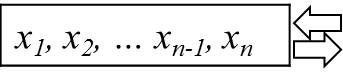
\includegraphics[width=0.25\textwidth]{img/absstack1.png}
\end{center}

Here is a more complex example, showing the effect of several steps on the
state of assignable variables and allocated memory, where the stack
data structure resides:
\begin{center}
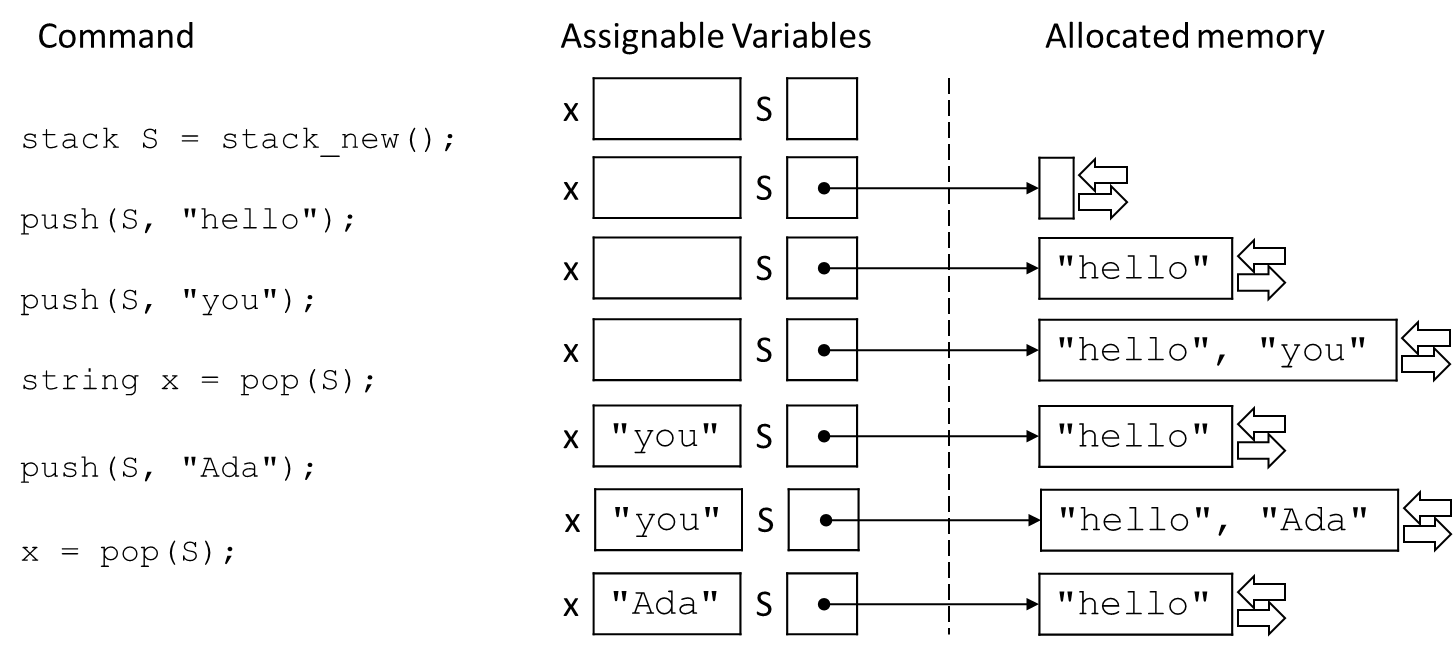
\includegraphics[width=0.99\textwidth]{img/absstack-ill.png}
\end{center}
Remember that we think of the assignable {\tt S} like a pointer or an
array: it is not literally an arrow but a number representing the
address of the in-memory representation of the stack.


%\section{Structs}
%
%A \emph{struct} is just an aggregate type, consisting of several data
%elements stored together of potentially different types.  Compare this
%to arrays, which is an aggregate of elements of the same type.
%Structs must be explicitly declared.  For example, a struct
%representing a point in two-dimensional space (such as the location of
%a pixel in an image), could be declared as
%\begin{lstlisting}[numbers=left]
%struct point {
%  int x;
%  int y;
%  bool visited;
%};
%\end{lstlisting}
%Here $x$, $y$, and $\mathit{visited}$ are not variables, but
%\emph{fields} of the struct.  The declaration expresses that every
%point has $x$ and $y$ fields, intended to represent its coordinates,
%and a $\mathit{visited}$ field that might be used in a program, say,
%to computed shortest paths between points.
%
%Structs do not necessarily fit into a machine word because they can
%have arbitrarily many components, so they must be allocated on the
%heap (in memory, just like arrays).  This is true if they happen to be
%small enough to fit into a word in order to maintain a uniform and
%simple language.
%
%How, then, do we manipulate structs?  We use the same solution as for
%arrays: we manipulate them via their address in memory.  Instead of
%\lstinline'alloc_array' we call \lstinline'alloc' which returns a \emph{pointer}
%to the struct that has been allocated in memory.  Let's look at an
%example in coin.
%\begin{lstlisting}[language={[coin]C}]
%% coin coord.c0
%Coin 0.3.0 'Nickel'(r103, Mon Aug 27 15:30:29 EDT 2012)
%Type `#help' for help or `#quit' to exit.
%--> struct point* p = alloc(struct point);
%p is 0xFF4FFF80 (struct point*)
%-->
%\end{lstlisting}
%We can access the fields of a structs, for reading or writing,
%through the notation \lstinline'p -> f' where $p$ is a pointer to
%a struct, and $f$ is the name of a field in that struct.
%Continuing above, let's see what the default values are
%in the allocated memory.
%\begin{lstlisting}[language={[coin]C}]
%--> p->x;
%0 (int)
%--> p->y;
%0 (int)
%--> p->visited;
%false (bool)
%-->
%\end{lstlisting}
%We can write to the fields of a struct by using the arrow
%notation on the left-hand side of an assignment.
%\begin{lstlisting}[language={[coin]C}]
%--> p->x = 438;
%(*(p)).x is 438 (int)
%--> p->x;
%438 (int)
%-->
%\end{lstlisting}

%% \section{One Stack Implementation (With Arrays)}

%% Any programming language is going to come with certain data structures
%% ``built-in.'' Arrays, the only really complex data structure we have
%% used so far in this class, are one example in C0. Other data
%% structures, like stacks and queues, need to be constructed
%% using more primitive language features.

%% We will get to a more proper implementation of stacks in the next
%% lecture, using linked lists.  For this lecture we will implement
%% stacks by using the familiar arrays that we have already been using so
%% far in this class.

%% The idea is to put all data elements in an array and maintain an
%% integer \lstinline'top', which is the index where we read off elements.
%% \begin{center}
%% 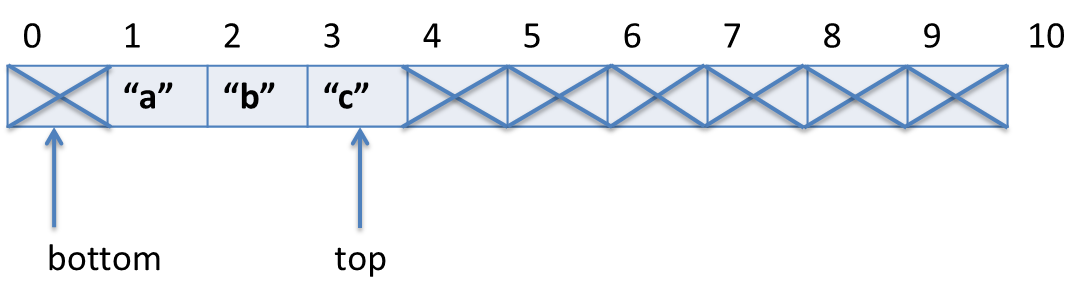
\includegraphics[width=0.85\textwidth]{img/arraystack1.png}
%% \end{center}
%% To help identify the similarities with the queue implementation, we
%% decide to also remember an integer \lstinline'bottom', which is the index of the
%% bottom of the stack.  (The bottom will, in fact, remain 0.)

%% With this design decision,
%% we do not have to handle the bottom of the stack much different than
%% any other element on the stack. The difference is that the data at the
%% bottom of the stack is meaningless and will not be used in our
%% implementation.

%% There appears to be a very big limitation to this design of stacks:
%% our stack can't contain more than 9 elements, like a pile of books on
%% our desk that cannot grow too high lest it reach the ceiling or fall
%% over. There are multiple solutions to this problem, but for this
%% lecture we will be content to work with stacks that have a limited
%% maximum capacity.

%% \subsection{Structs and data structure invariants}

%% Currently, our picture of a stack includes three different things: an
%% array containing the data, an integer indicating where the top
%% is, and an integer indicating where the bottom is. This is similar to
%% the situation in Homework 1 where we had data (an array of pixels) and
%% two integers, a width and a height.

%% C0 has a feature that allows us to bundle
%% these things up into a {\tt struct} rather than passing around all the
%% pieces separately.
%% We define:
%% \begin{lstlisting}[number=left]
%% struct stack_header {
%%   elem[] data;
%%   int top;
%%   int bottom;
%% };
%% typedef struct stack_header* stack;
%% \end{lstlisting}

%% What this notation means exactly, and especially what the part with
%% \lstinline'struct stack_header*' is all about, will be explained in the next
%% lecture.  (These are pointers and it is crucial to understand them,
%% but we defer this topic for now.)  For now, it is
%% sufficient to think of this as providing a notation for bundling
%% aggregate data. When we have a struct \lstinline'S' of type \lstinline'stack', we
%% can refer to the data as \lstinline'S->data', the integer representing
%% the top of the stack as \lstinline'S->top', and the integer representing
%% the bottom of the stack as \lstinline'S->bottom'.

%% When does a struct of this type represent a valid stack?  Whenever we
%% define a new data type representation we should first think about the
%% data structure invariants.  Making these explicit is important as we
%% think about and write the pre- and postconditions for functions that
%% implement the interface.  Here, it is a simple check of making sure
%% that the \lstinline'bottom' and \lstinline'top' indices are in the range of the
%% array and that \lstinline'bottom' stays at 0, where we expect it to be.

%% \begin{lstlisting}[numbers=left]
%% bool is_stack(stack S)
%% {
%%   if (!(S->bottom == 0)) return false;
%%   if (!(S->bottom <= S->top)) return false;
%%   //@assert S->top < \length(S->data);
%%   return true;
%% }
%% \end{lstlisting}

%% \noindent
%% {\bf WARNING:} This specification function is missing something very
%% important (a check for \lstinline'NULL') --- we will return to this next
%% time!

%% When we write specification functions, we use a style of repeatedly saying
%% \begin{lstlisting}[numbers=left]
%%   if (!(some invariant of the data structure)) return false;
%% \end{lstlisting}
%% so that we can read off the invariants of the data structure. A
%% specification function like \lstinline|is_stack| should be safe --- it
%% should only ever return \lstinline'true' or \lstinline'false' or raise an
%% assertion violation --- and if possible it should avoid raising an
%% assertion violation. Assertion violations are sometimes unavoidable
%% because we can only check the length of an array inside of the
%% assertion language.

%% \subsection{Checking for emptiness}

%% To check if the stack is empty, we only need to check whether
%% \lstinline'top' and \lstinline'bottom' are the same number.
%% \begin{lstlisting}[numbers=left]
%% bool stack_empty(stack S)
%% //@requires is_stack(S);
%% {
%%   return S->top == S->bottom;
%% }
%% \end{lstlisting}

%% \newpage
%% \subsection{Popping from a stack}
%% To pop an element from the stack we just look up the data that is stored at the position indicated by the \lstinline'top' field of the stack in the array \lstinline'S->data' of the \lstinline'data' field of the stack.
%% To indicate that this element has now been removed from the stack, we decrement the \lstinline'top' field of the stack.
%% We go from
%% \begin{center}
%% 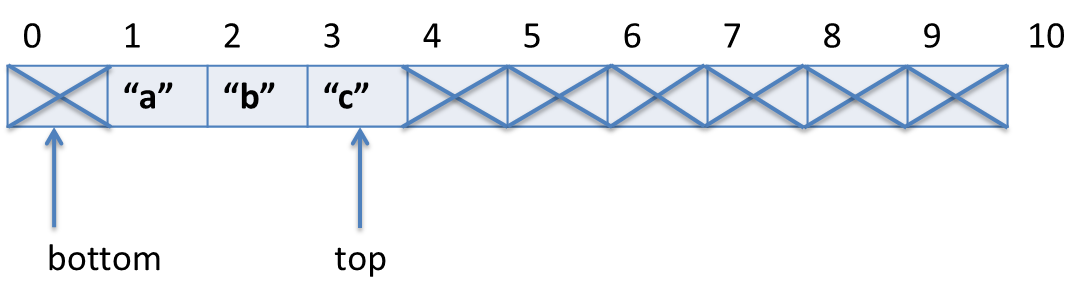
\includegraphics[width=0.85\textwidth]{img/arraystack1.png}
%% \end{center}
%% to
%% \begin{center}
%% 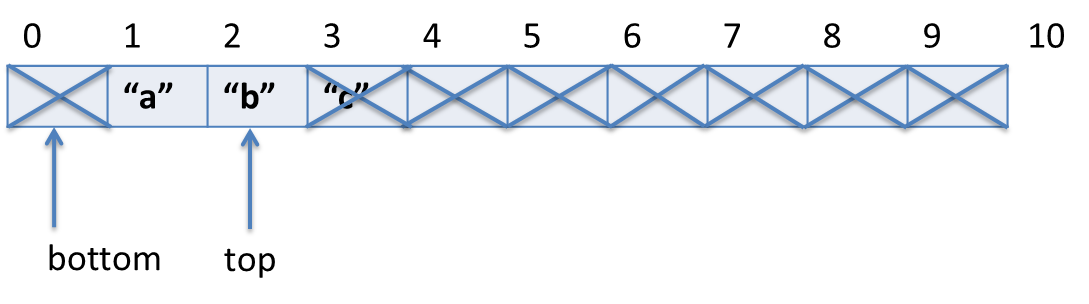
\includegraphics[width=0.85\textwidth]{img/arraystack2.png}
%% \end{center}
%% The \lstinline|"c"| can still be present in the array at position 3, but it
%% is now a part of the array that we don't care about, which we indicate by
%% putting an \lstinline|X| over it.
%% In code, popping looks like this:
%% \begin{lstlisting}[numbers=left]
%% elem pop(stack S)
%% //@requires is_stack(S);
%% //@requires !stack_empty(S);
%% //@ensures is_stack(S);
%% {
%%   elem r = S->data[S->top];
%%   S->top--;
%%   return r;
%% }
%% \end{lstlisting}
%% Notice that contracts are cumulative. Since we already indicated
%% \begin{lstlisting}[numbers=left]
%% //@requires !stack_empty(S);
%% \end{lstlisting}
%% in the interface of \lstinline'pop', we would not have to repeat this requires clause in
%% the implementation. We repeat it regardless to emphasize its importance.

%% \newpage
%% \subsection{Pushing onto a stack}

%% To push an element onto the stack, we increment the \lstinline'top' field
%% of the stack to reflect that there are more elements on the stack.
%% And then we put the element \lstinline'e' into the
%% array \lstinline'S->data' at position \lstinline'top'.  While
%% this is simple, it is still a good idea to draw a diagram.  We go from
%% \begin{center}
%% 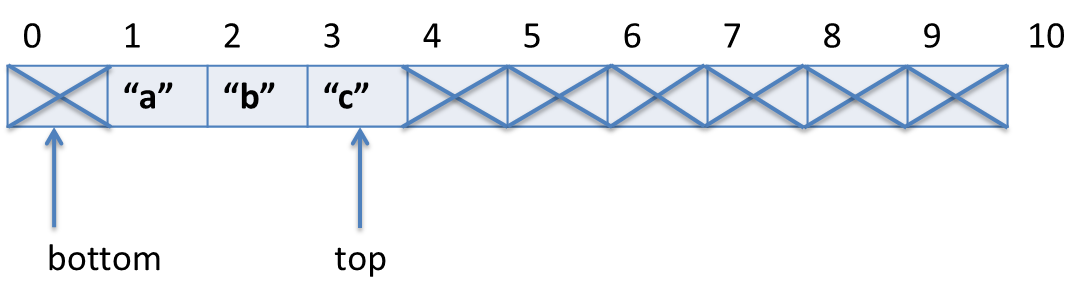
\includegraphics[width=0.99\textwidth]{img/arraystack1.png}
%% \end{center}
%% to
%% \begin{center}
%% 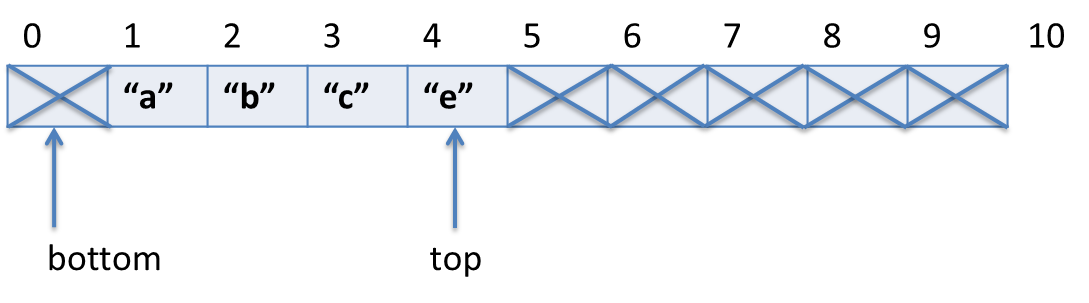
\includegraphics[width=0.85\textwidth]{img/arraystack3.png}
%% \end{center}

%% In code:
%% \begin{lstlisting}[numbers=left]
%% void push(stack S, elem e)
%% //@requires is_stack(S);
%% //@ensures is_stack(S);
%% {
%%   S->top++;
%%   S->data[S->top] = e;
%% }
%% \end{lstlisting}

%% Why is the array access \lstinline'S->data[S->top]' safe? Is it even safe?
%% At this point, it is important to note that it is not safe if we ever
%% try to push more elements on the stack than we have reserved space
%% for.  We fully address this shortcoming of our stack implementation in
%% the next lecture.  What we can do right now to address the issue is to
%% redesign the \lstinline'struct stack_header' by adding a \lstinline'capacity'
%% field that remembers the length of the array of the \lstinline'data' field:
%% \begin{lstlisting}[numbers=left]
%% struct stack_header {
%%   elem[] data;
%%   int top;
%%   int bottom;
%%   int capacity;           // capacity == \length(data);
%% };
%% typedef struct stack_header* stack;
%% \end{lstlisting}
%% Giving us the following updated view of array-based stacks:
%% \begin{center}
%% 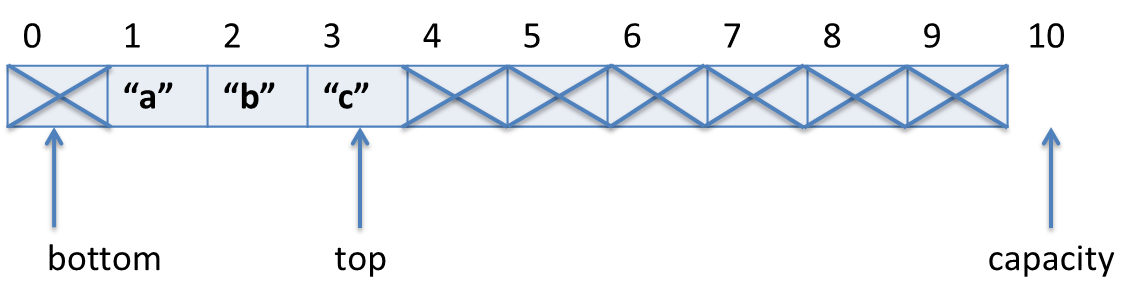
\includegraphics[width=0.85\textwidth]{img/arraystack4.png}
%% \end{center}

%% The comment that \lstinline'capacity == '\length{(data)} is helpful for
%% indicating what the intent of \lstinline'capacity' is, but it is preferable
%% for us to modify our \lstinline'is_stack' function to account for the
%% change. (The {\bf WARNING} from before still applies here.)

%% \begin{lstlisting}[numbers=left]
%% bool is_stack(stack S)
%% {
%%   if (!(S->bottom == 0)) return false;
%%   if (!(S->bottom <= S->top)) return false;
%%   if (!(S->top < S->capacity)) return false;
%%   //@assert S->capacity == \length(S->data);
%%   return true;
%% }
%% \end{lstlisting}


%% With a \lstinline'capacity' in hand, we check for sufficient space with an
%% explicit assert statement before we try to access the array or change
%% \lstinline'top'.

%% \begin{lstlisting}[numbers=left]
%% void push(stack S, elem e)
%% //@requires is_stack(S);
%% //@ensures is_stack(S);
%% {
%%   assert(S->top < S->capacity - 1);  // otherwise no space left
%%   S->top++;
%%   S->data[S->top] = e;
%% }
%% \end{lstlisting}

%%  This assertion can indeed fail if the client tries to push too many
%%  elements on the stack, which is why we use a \emph{hard assert} -- an
%%  assertion that will run whether or not we compile with \lstinline'-d'. The
%%  alternative would be to expose the capacity of the stack to the user
%%  with a \lstinline'stack_full' function and then add a precondition
%%  \lstinline'//@requires !stack_full(S)' to our \lstinline'push()' function.

%% \subsection{Creating a new stack}

%% For creating a new stack, we allocate a \lstinline'struct stack_header' and initialize the
%% \lstinline'top' and \lstinline'bottom' numbers to 0.
%% \begin{lstlisting}[numbers=left]
%% stack stack_new()
%% //@ensures stack_empty(\result);
%% //@ensures is_stack(\result);
%% {
%%   stack S = alloc(struct stack_header);
%%   S->bottom = 0;
%%   S->top = 0;
%%   S->capacity = 090;               // arbitrary resource bound
%%   S->data = alloc_array(elem, S->capacity);
%%   return S;
%% }
%% \end{lstlisting}
%% As shown above, we also need to allocate an array \lstinline'data' to store the elements in.
%% At this point, at the latest, we realize a downside of our stack implementation.
%% If we want to implement stacks in arrays in the simple way that we just did, the trouble is that we need to decide its capacity ahead of time. That is, we need to decide how many elements at maximum will ever be allowed in the stack at the same time.
%% Here, we arbitrarily choose the capacity 090, but this gives us a rather poor implementation of stacks in case the client needs to store more data.
%% We will see how to solve this issue with a better implementation of stacks in the next lecture.

%% This completes the implementation of stacks, which are a very simple
%% and pervasive data structure.

\section{Abstraction}
\label{sec:stackqueue:abstraction}
\TAGS{interface, stack}

An important point about formulating a precise interface to a data
structure like a stack is to achieve \emph{abstraction}.  This means
that as a client of the data structure we can only use the functions
in the interface.  In particular, we are not permitted to use or even
know about details of the implementation of stacks.

Let's consider an example of a client-side program.  We would like to
examine the element at the top of the stack without removing it from the
stack.  Such a function would have the declaration
\begin{lstlisting}[language={[C0]C}]
string peek(stack_t S)
/*@requires S != NULL && !stack_empty(S); @*/ ;
\end{lstlisting}
If we knew how stacks were implemented, we might be able to implement,
as clients of the stack data structure, something like this:
\begin{lstlisting}[language={[C0]C}, numbers=left]
string peek(stack_t S)
//@requires is_stack(S) && !stack_empty(S);
{
  return S->data[S->top];
}
\end{lstlisting}
However, \emph{we don't know how stacks are implemented, so we cannot
  do this}. As clients of the stack data structure, we only know about
the functions provided by the interface.  However, it is possible to
implement the peek operation correctly \emph{without violating the
  abstraction}!

The idea is that we pop the top element off the stack, remember it
in a temporary variable, and then push it back onto the stack before we return.
\begin{lstlisting}[language={[C0]C}, numbers=left]
string peek(stack_t S)
//@requires S != NULL && !stack_empty(S);
{
  string x = pop(S);
  push(S, x);
  return x;
}
\end{lstlisting}

Depending on the implementation of stacks, this might be less
efficient than a library-side implementation of peek.  However, as
long as \lstinline'push' and \lstinline'pop' are still a constant-time
operations, \lstinline'peek' will still be constant time ($O(1)$).


\section{Computing the Size of a Stack}
\label{sec:stackqueue:size}
\TAGS{aliasing, interface, stack}

Let's exercise our data structure once more by considering how to
implement a function that returns the size of a stack, using only the
interface.  In the next lecture we'll consider how to do this on the
library's side, exploiting the data representation.

Here's the signature of a client-side implementation.
\begin{lstlisting}[language={[C0]C}]
int stack_size(stack_t S)
/*@requires S != NULL;   @*/
/*@ensures \result >= 0; @*/ ;
\end{lstlisting}

\newpage
We encourage you to consider this problem and program it before you
read on.

First we reassure ourselves that it will not be a simple operation.
We do not have access to the array (in fact, as the client, we cannot
know that there is an array), so the only thing we can do is pop all
the elements off the stack.  This can be accomplished with a
while-loop that finishes as soon as the stack is empty.
\begin{lstlisting}[language={[C0]C}, numbers=left]
int stack_size(stack_t S)
//@requires S != NULL;
//@ensures \result >= 0;
{
  int count = 0;
  while (!stack_empty(S)) {
    pop(S);
    count++;
  }
  return count;
}
\end{lstlisting}
However, this function has a \emph{big} problem: in order to compute
the size we have to destroy the stack!  Clearly, there may be
situations where we would like to know the number of elements in a
stack without deleting all of its elements.  Fortunately, we can use
the idea from the \lstinline'peek' function in amplified form: we maintain
a new \emph{temporary stack} $T$ to hold the elements we pop from $S$.
Once we are done counting, we push them back onto $S$ to repair the
damage.
\clearpage
\begin{lstlisting}[language={[C0]C}, numbers=left]
int stack_size(stack_t S)
//@requires S != NULL;
//@ensures \result >= 0;
{
  stack_t T = stack_new();
  int count = 0;
  while (!stack_empty(S)) {
    push(T, pop(S));
    count++;
  }
  while (!stack_empty(T)) {
    push(S, pop(T));
  }
  return count;
}
\end{lstlisting}
The complexity of this function is clearly $O(n)$, where $n$ is the
number of elements in the stack $S$, since we traverse each while loop
$n$ times, and perform a constant number of operations in the body of
both loops.  For that, we need to know that \lstinline'push' and \lstinline'pop'
are constant time ($O(1)$).

A library-side implementation of \lstinline'stack_size' can be done in
$O(1)$, but we won't consider that today.

%%\section{Exploiting Abstraction and Data Structure Invariants}
%%
%%The \lstinline'stack_size' operation from the previous
%%section is still a linear-time operation ($O(n)$),
%%because we have to traverse the whole linked list.
%%
%%Can we do better?  Yes!  We can make it constant time, which may seem
%%like magic.  Think about it before you read on.
%%
%%\clearpage
%%The trick is to introduce a new field into the header struct of a
%%stack which contains the size.  We initialize it to 0 when we create
%%the stack.  Every time we push an element onto the stack we increment
%%the size field, every time we pop an element from the stack we
%%decrement the size field.  You can find the full code in the file
%%\href{http://www.cs.cmu.edu/~fp/courses/15122-f12/09-stacks/stacks.c0}{stacks.c0}.
%%Here we show only the new header structure definition and the
%%\lstinline'is_stack' function which checks the invariants.
%%
%%\begin{lstlisting}[numbers=left]
%%struct stack_header {
%%  list* top;
%%  list* bottom;
%%  int size;    /* num of elements in stack */
%%};
%%
%%bool is_stack(stack S) {
%%  if (S == NULL) return false;
%%  if (S->top == NULL || S->bottom == NULL) return false;
%%  if (!is_segment(S->top, S->bottom)) return false;
%%  if (S->size != list_size(S->top, S->bottom)) return false;
%%  return true;
%%}
%%
%%int stack_size(stack S)
%%//@requires is_stack(S);
%%{
%%  return S->size;
%%}
%%\end{lstlisting}
%%
%%Note that in \lstinline'is_stack' we still use the function
%%\lstinline'list_size' we wrote before, but now it is just used to check
%%that the data structure invariants are preserved.  When
%%we actually retrieve the size we just look at the field.
%%
%%Why is this correct?  Here we can bring the power of abstraction to
%%bear.  Since no client can directly access the size field, or the top
%%or bottom pointers, we only have to show that each of the operations
%%listed in the interface maintains the invariant.  And this is the
%%case, if we have correct push and pop functions.  For example,
%%\clearpage
%%\begin{lstlisting}[numbers=left]
%%elem pop(stack S)
%%//@requires is_stack(S);
%%//@requires !stack_empty(S);
%%//@ensures is_stack(S);
%%{
%%  elem e = S->top->data;
%%  S->top = S->top->next;
%%  (S->size)--;
%%  return e;
%%}
%%\end{lstlisting}


\section{The Queue Interface}
\label{sec:stackqueue:queue-interface}
\TAGS{complexity, interface, queue}

A \emph{queue} is a data structure where we add elements at the back
and remove elements from the front.  In that way a queue is like
``waiting in line'': the first one to be added to the queue will be
the first one to be removed from the queue.  This is also called a
FIFO (First In First Out) data structure.  Queues are common in many
applications.  For example, when we read a book from a file, it would
be natural to store the words in a queue so that when we are finished
reading the file the words are in the order they appear in the book.
Another common example are buffers for network communication that
temporarily store packets of data arriving on a network port.
Generally speaking, we want to process them in the order they arrive.

\clearpage
\noindent
Here is our interface:
\begin{lstlisting}[language={[C0]C}]
// typedef ______* queue_t;

bool queue_empty(queue_t Q)       /* O(1) */
  /*@requires Q != NULL; @*/;

queue_t queue_new()               /* O(1) */
  /*@ensures \result != NULL; @*/
  /*@ensures queue_empty(\result); @*/;

void enq(queue_t Q, string e)     /* O(1) */
  /*@requires Q != NULL; @*/;

string deq(queue_t Q)             /* O(1) */
  /*@requires Q != NULL; @*/
  /*@requires !queue_empty(Q); @*/ ;
\end{lstlisting}
Dequeuing is only possible on non-empty queues, which we indicate
by a \requires{} contract in the interface.

Again, we can write out this interface without committing to an
implementation of queues.  In particular, the type \lstinline'queue_t'
remains \emph{abstract} in the sense that we have not given its
definition.  This is important so that different implementations of
the functions in this interface can choose different representations.
Clients of this data structure should not care about the internals of
the implementation.  In fact, they should not be allowed to access
them at all and operate on queues only through the functions in this
interface.  Some languages with strong module systems enforce such
abstraction rigorously.  In $C$, it is mostly a matter of adhering to
conventions.


\section{Using the Queue Interface}
\label{sec:stackqueue:using-queues}
\TAGS{queue}

We play through some simple examples to illustrate the idea
of a queue and how to use the interface above.  We write
a queue as
$$
x_1, x_2, \ldots, x_n
$$
where $x_1$ is the \emph{front} of the queue and
$x_n$ is the \emph{back} of the queue.  We \emph{enqueue}
elements in the back and \emph{dequeue} them from the
front. If we want to emphasize this, we can draw queues like this:
\begin{center}
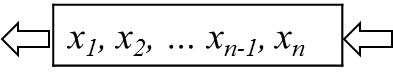
\includegraphics[width=0.3\textwidth]{img/absqueue.png}
\end{center}

Here's a trace of the queues in action:
\begin{center}
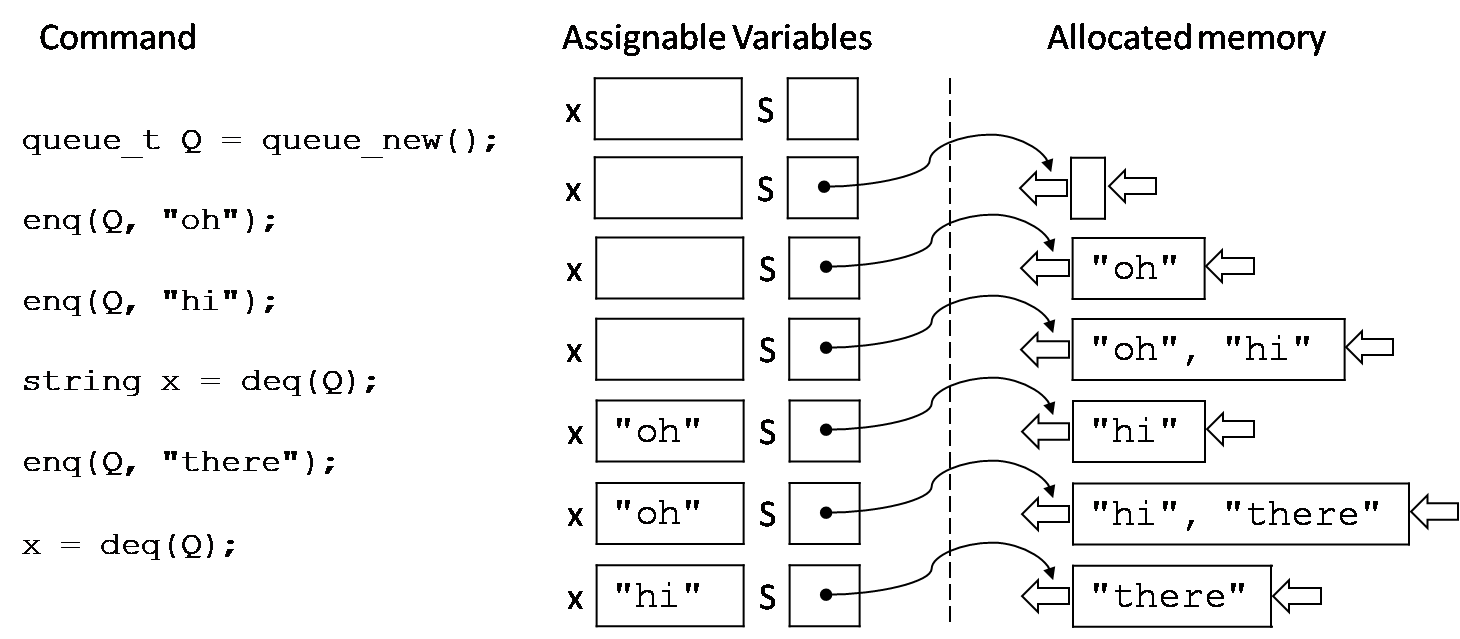
\includegraphics[width=0.99\textwidth]{img/absqueue-ill.png}
\end{center}


\section{Copying a Queue Using Its Interface}
\label{sec:stackqueue:copying-queue}
\TAGS{aliasing, interface, queue}

Suppose we have a queue $Q$ and want to obtain a copy of it.  That is,
we want to create a new queue $C$ and implement an algorithm that will
make sure that $Q$ and $C$ have the same elements and in the same
order.
%Besides, we want to make sure that, after running the copying algorithm, the queue $Q$ has exactly the same elements as it used to have before the algorithm.
How can we do that?  Before you read on, see if you can figure it out
for yourself.

\clearpage%\rule{\textwidth}{1pt}

The first thing to note is that
\begin{lstlisting}[language={[C0]C}]
  queue_t C = Q;
\end{lstlisting}
will not have the effect of copying the queue $Q$ into a new queue
$C$. This assignment makes $C$ and $Q$ aliases, so if we change one of
the two, for example enqueue an element into $C$, then the other queue
will have changed as well.  Just as for the case of stack size, we
need to implement a function for copying the data.

The queue interface provides functions that allow us to dequeue data
from the queue, which we can do as long as the queue is not empty.  So
we create a new queue $C$. Then we read all data from queue $Q$ and
put it into the new queue $C$.
\begin{lstlisting}[language={[C0]C}, numbers=left]
  queue_t C = queue_new();
  while (!queue_empty(Q)) {
    enq(C, deq(Q));
  }
  //@assert queue_empty(Q);
\end{lstlisting}
Now the new queue $C$ will contain all data that was previously in
$Q$, so $C$ is a copy of what used to be in $Q$.  But there is a
problem with this approach.  Before you read on, can you find out
which problem?

\clearpage
Queue $C$ now is a copy of what used to be in $Q$ before we started
copying. But our copying process was destructive! By dequeuing all
elements from $Q$ to put them into $C$, $Q$ has now become empty.  In
fact, our assertion at the end of the above loop even indicated
\lstinline'queue_empty(Q)'.  So what we need to do is put all data
back into $Q$ when we are done copying it all into $C$.  But where do
we get it from?  We could read it from the copy $C$ to put it back
into $Q$, but, after that, the copy $C$ would be empty, so we are back
to where we started from.  Can you figure out how to copy all data
into $C$ and make sure that it also ends up in $Q$?  Before you read
on, try to find a solution for yourself.

\clearpage
We could try to enqueue all data that we have read from $Q$ back into
$Q$ before putting it into $C$.
\begin{lstlisting}[language={[C0]C}, numbers=left]
  queue_t C = queue_new();
  while (!queue_empty(Q)) {
    string s = deq(Q);
    enq(Q, s);
    enq(C, s);
  }
  //@assert queue_empty(Q);
\end{lstlisting}
But there is something very fundamentally wrong with this idea.
Can you figure it out?

\clearpage
The problem with the above attempt is that the loop will never
terminate unless $Q$ is empty to begin with.  For every element that
the loop body dequeues from $Q$, it enqueues one element back into
$Q$.  That way, $Q$ will always have the same number of elements and
will never become empty.  Therefore, we must go back to our original
strategy and first read all elements from $Q$.  But instead of putting
them into $C$, we will put them into a third queue $T$ for temporary
storage.  Then we will read all elements from the temporary storage
$T$ and enqueue them into both the copy $C$ \emph{and} back into the
original queue $Q$.  At the end of this process, the temporary queue
$T$ will be empty, which is fine, because we will not need it any
longer.  But both the copy $C$ and the original queue $Q$ will be
replenished with all the elements that $Q$ had originally.  And $C$
will be a copy of $Q$.
\begin{lstlisting}[language={[C0]C}, numbers=left]
queue_t queue_copy(queue_t Q)
//@requires Q != NULL;
//@ensures \result != NULL;
{
  queue_t T = queue_new();
  while (!queue_empty(Q)) {
    enq(T, deq(Q));
  }
  //@assert queue_empty(Q);
  queue_t C = queue_new();
  while (!queue_empty(T)) {
    string s = deq(T);
    enq(Q, s);
    enq(C, s);
  }
  //@assert queue_empty(T);
  return C;
}
\end{lstlisting}
For example, when \lstinline'queue_copy' returns, neither $C$ nor $Q$
will be empty.  Except if $Q$ was empty to begin with, in which case
both $C$ and $Q$ will still be empty in the end.

%% \clearpage
%% \section{The Queue Implementation}

%% In this lecture, we implement the queue using an array, similar to how we have implemented stacks in this lecture.
%% \begin{center}
%% 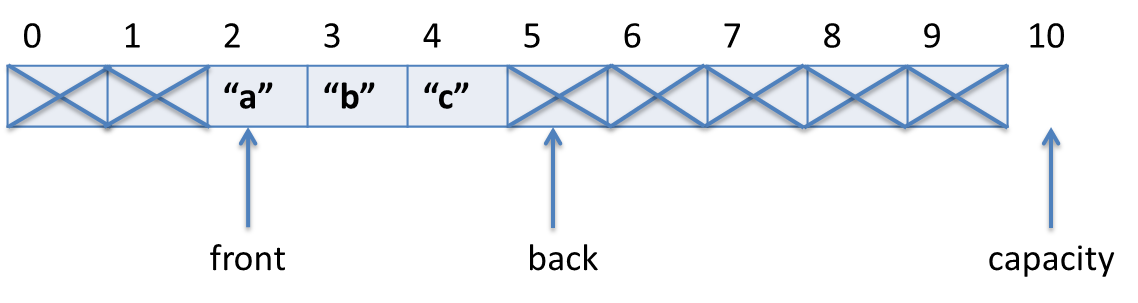
\includegraphics[width=0.85\textwidth]{img/arrayqueue1.png}
%% \end{center}

%% A queue is implemented as a struct with a \lstinline'front' and \lstinline'back'
%% field.  The \lstinline'front' field is the index of the front of the queue, the
%% \lstinline'back' field is the index of the back of the queue.  We need both so that we can dequeue (at the front) and enqueue (back).

%% In the stack, we did not use anything outside the range $({\it
%%   bottom}, \emph{top}]$, and for queues, we do not use anything
%% outside the range $[\emph{front}, \emph{back})$.
%% Again, we mark this in diagrams with an \lstinline'X'.
%% %In arrays, we often work with the length which is one greater than the
%% %index of the last element in the array.  In queues, we use a similar
%% %strategy, making sure the \lstinline'back' pointer points to one element
%% %past the end of the queue.  Unlike arrays, there must be something in
%% %memory for the pointer to refer to, so there is always one extra
%% %element at the end of the queue which does not have valid data or
%% %\lstinline'next' pointer.  We have indicated this in the diagram by writing
%% %\lstinline'X'.

%% The above picture yields the following definition, where we
%% will again remember the capacity of the queue, i.e., the length of
%% the array stored in the \lstinline'data' field.
%% \begin{lstlisting}[numbers=left]
%% struct queue_header {
%%   elem[] data;
%%   int front;
%%   int back;
%%   int capacity;
%% };
%% typedef struct queue_header* queue;
%% \end{lstlisting}
%% %We call this a \emph{header} because it doesn't hold any elements of
%% %the queue, just pointers to the linked list that really holds them.
%% %The type definition allows us to use \lstinline'queue' as a type that
%% %represents a \emph{pointer to a queue header}.  We define it this way
%% %so we can hide the true implementation of queues from the client and
%% %just call it an element of type \lstinline'queue'.

%% When does a struct of this type represent a valid queue?  In fact,
%% whenever we define a new data type representation we should first
%% think about the data structure invariants.  Making these explicit is
%% important as we think about and write the pre- and postconditions for
%% functions that implement the interface.

%% What we need here is simply that the \lstinline'front'
%% and \lstinline'back' are within the array bounds for array \lstinline'data' and that the capacity is not too small.
%% The \lstinline'back' of the queue is not used (marked \lstinline'X') but in the array, so we decide to require that the capacity of a queue be at least 2 to make sure we can store at least one element.
%% (The {\bf WARNING} about NULL still applies here.)
%% \begin{lstlisting}[numbers=left]
%% bool is_queue(queue Q)
%% {
%%   if (Q->capacity < 2) return false;
%%   if (Q->front < 0 || Q->front >= Q->capacity) return false;
%%   if (Q->back < 0 || Q->back >= Q->capacity) return false;
%%   //@assert Q->capacity == \length(Q->data);
%%   return true;
%% }
%% \end{lstlisting}

%% To check if the queue is empty we just compare its front and back.
%% If they are equal, the queue is empty; otherwise it is not.  We
%% require that we are being passed a valid queue.  Generally, when
%% working with a data structure, we should always require and ensure
%% that its invariants are satisifed in the pre- and post-conditions of
%% the functions that manipulate it.  Inside the function, we will
%% generally temporarily violate the invariants.

%% % When programming with shared memory concurrency, this can create a lot
%% % of difficulties (but not in C0).

%% \begin{lstlisting}[numbers=left]
%% bool queue_empty(queue Q)
%% //@requires is_queue(Q);
%% {
%%   return Q->front == Q->back;
%% }
%% \end{lstlisting}

%% To  dequeue an element, we only need to
%% increment the field \lstinline'front', which represents the index in \lstinline'data' of the front of the queue.
%% To emphasize that we never use portions of the array outside the \lstinline'front' to \lstinline'back' range, we first save the dequeued
%% element in a temporary variable so we can return it later.  In
%% diagrams:
%% \begin{center}
%% 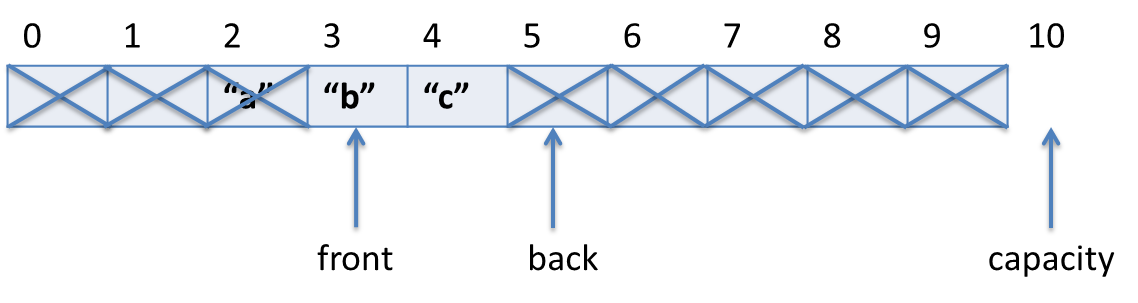
\includegraphics[width=0.85\textwidth]{img/arrayqueue2.png}
%% \end{center}

%% \clearpage
%% And in code:
%% \begin{lstlisting}[numbers=left]
%% elem deq(queue Q)
%% //@requires is_queue(Q);
%% //@requires !queue_empty(Q);
%% //@ensures is_queue(Q);
%% {
%%   elem e = Q->data[Q->front];
%%   Q->front++;
%%   return e;
%% }
%% \end{lstlisting}
%% %Q->front = (Q->front + 1) % Q->capacity;

%% To enqueue something, that is, add a new item to the back of
%% the queue, we just write the data (here: a string) into the
%% extra element at the back, and increment \lstinline'back'.  You should draw
%% yourself a diagram before you write this kind of code.
%% Here is a before-and-after diagram for inserting \lstinline'"e"':
%% \begin{center}
%% 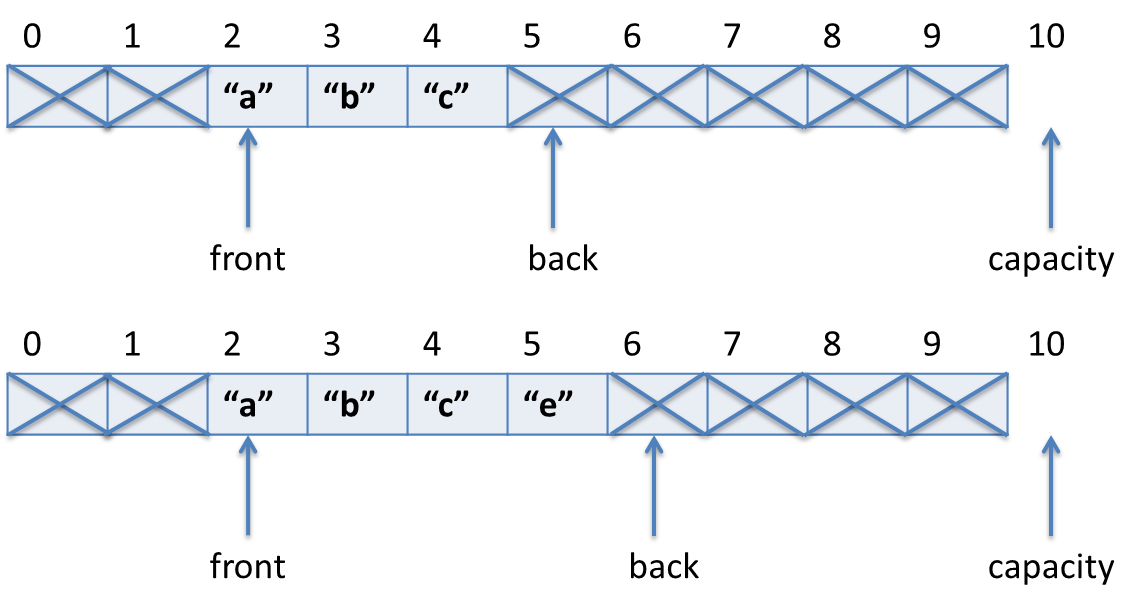
\includegraphics[width=0.85\textwidth]{img/arrayqueue3.png}
%% \end{center}

%% In code:
%% \begin{lstlisting}[numbers=left]
%% void enq(queue Q, string s)
%% //@requires is_queue(Q);
%% //@ensures is_queue(Q);
%% //@ensures !queue_empty(Q);
%% {
%%   assert(Q->back < Q->capacity-1);  // otherwise out of resources
%%   Q->data[Q->back] = e;
%%   Q->back++;
%% }
%% \end{lstlisting}
%% %  Q->back = (Q->back + 1) % Q->capacity;
%% % The invariant marked \emph{internal} is one that only makes sense
%% % in the context of the present implementation, but would not be
%% % meaningful to a client.


%% To obtain a new empty queue, we allocate a queue header struct and
%% initialize both \lstinline'front' and \lstinline'back' to 0, the first element of the array.  We
%% do not initialize the elements in the array because its contents are
%% irrelevant until some data is put in.  It is good practice
%% to always initialize memory if we care about its contents, even
%% if it happens to be the same as the default value placed there.
%% \begin{lstlisting}[numbers=left]
%% queue queue_new()
%% //@ensures is_queue(\result);
%% //@ensures queue_empty(\result);
%% {
%%   queue Q = alloc(struct queue_header);
%%   Q->front = 0;
%%   Q->back = 0;
%%   Q->capacity = 100;
%%   Q->data = alloc_array(elem, Q->capacity);
%%   return Q;
%% }
%% \end{lstlisting}
%% %Let's take one of these lines apart.  Why does
%% %\begin{lstlisting}[numbers=left]
%% %  queue Q = alloc(struct queue_header);
%% %\end{lstlisting}
%% %make sense?  According to the definition of \lstinline'alloc',
%% %we might expect
%% %\begin{lstlisting}[numbers=left]
%% %  struct queue_header* Q = alloc(struct queue_header);
%% %\end{lstlisting}
%% %since allocation returns the address of what we allocated.
%% %Fortunately, we defined \lstinline'queue' to be a short-hand
%% %for \lstinline'struct queue_header*' so all is well.

%% Observe that, unlike the queue implementation, the queue interface only uses a single contract: that \lstinline'deq' requires a non-empty queue to work.
%% The queue implementation has several additional implementation contracts.
%% All queue implementation functions use \lstinline'is_queue(Q)' in their requires and ensures contract.
%% The only exception is the \lstinline'queue_new' implementation, which ensures the analogue \lstinline'is_queue(\result)' instead.
%% These \lstinline'is_queue' contracts do not appear in the queue interface because \lstinline'is_queue'  itself does not appear in the interface, because it is an \emph{internal data structure invariant}.
%% If the client obeys the interface abstraction, all he can do with queues is create them via \lstinline'queue_new' and then pass them to the various queue operations in the interface.
%% At no point in this process does the client have the opportunity to tamper with the queue data structure to make it fail \lstinline'is_queue', unless the client violates the interface.

%% But there are other additional contracts in the queue implementation, which we want to use to check our implementation, and they still are not part of the interface.
%% For example. we could have included the following additional contracts in the interface
%% \begin{lstlisting}[numbers=left]
%% queue queue_new()          /* O(1), create new empty queue */
%% //@ensures queue_empty(\result);
%%   ;
%% void enq(queue Q, elem s)  /* O(1), add item at back */
%% //@ensures !queue_empty(Q);
%%   ;
%% \end{lstlisting}
%% Those contracts need to hold for all queue implementations.
%% Why did we decide not to include them?
%% The reason is that there are not many situations in which this knowledge about queues is useful, because we rarely want to dequeue an element right after enqueueing it.
%% This is in contrast to the \lstinline'//@requires !queue_empty(Q)' contract of \lstinline'deq', which is critical for the client to know about, because he can only dequeue elements from non-empty queues and has to check for non-emptyness before calling \lstinline'deq'.

%% Similar observations hold for our rationale for designing the stack interface.

%% \section{Bounded versus Unbounded Stacks \& Queues}

%% Both the queue and the stack implementation that we have seen so far have a fundamental limitation. They are of bounded capacity. However large we allocate their \lstinline'data' arrays, there is a way of enqueuing elements into the queue or pushing elements onto the stack that requires more space than the array has had in the first place.
%% And if that happens, the \lstinline'enq' or \lstinline'push' operations will fail an assertion because of a resource bound that the client has no way of knowing about.
%% This is bad, because the client would have to expect that any of his \lstinline'enq' or \lstinline'push' operations might fail, because he does not know about the capacity of the queue and has no way of influencing this.

%% One way of solving this problem would be to add operations into the interface that make it possible to check whether a queue is full.
%% \begin{lstlisting}[numbers=left]
%% bool queue_full(queue Q);
%% \end{lstlisting}
%% Then we change the precondition of \lstinline'enq' to require that elements can only be enqueued if the queue is not full
%% \begin{lstlisting}[numbers=left]
%% void enq(queue Q, elem s)
%% //@requires !queue_full(Q)
%% ....
%% \end{lstlisting}
%% Similarly, we could add an operation to the interface of stacks to check whether the stack is full
%% \begin{lstlisting}[numbers=left]
%% bool stack_full(stack S);
%% \end{lstlisting}
%% And require that pushing is only possible if the stack is not full
%% \begin{lstlisting}[numbers=left]
%% void push(stack S, elem s)
%% //@requires !stack_full(S)
%% ....
%% \end{lstlisting}

%% The advantage of this design is that the client now has a way of checking whether there still is space in the stack/queue.
%% The downside, however, is that the client still does not have a way of increasing the capacity if he wants to store more data in it.

%% In the next lecture, we will see a better implementation of stacks and queues that does not have any of those capacity bounds. That implementation uses pointers and linked lists.

\clearpage
\section{Exercises}
\label{sec:stackqueue:exercises}

\begin{flex}
\begin{exercise}%[\opt{sample solution on page~\pageref{ex:stack_copy-reverse-solved}}]
\label{ex:stack_copy-reverse}
\exerciseTAGS{interface, stack}
The following code is intended to return an exact copy a stack.  It
falls short of this goal however.  What's wrong with the code?
\begin{lstlisting}[language={[C0]C}]
stack_t stack_copy(stack_t S)
//@requires S != NULL;
{
  stack_t tmp = stack_new();    // temporary stack
  stack_t copy = stack_new();   // stack to be returned

  // move all elements of S into tmp
  while (!stack_empty(S)) {
    string x = pop(S);
    push(copy, x);
    push(tmp, x);
  }

  while (!stack_empty(tmp))
    push(S, pop(tmp));

  return copy;
}
\end{lstlisting}
Implement a correct version of \lstinline'stack_copy' that does
return a copy of its input stack.
\end{exercise}

\begin{solution}\opt{\textbf{of exercise~\ref{ex:stack_copy-reverse}}}
\label{ex:stack_copy-reverse-solved}
  The returned copy of the input stack is in reverse order.  Here's a
  fixed version:
\begin{lstlisting}[language={[C0]C}]
stack_t stack_copy(stack_t S)
//@requires S != NULL;
{
  stack_t tmp = stack_new();    // temporary stack
  stack_t copy = stack_new();   // stack to be returned

  // move all elements of S into tmp
  // -- they will be in the reverse order
  while (!stack_empty(S))
    push(tmp, pop(S));
  //@assert stack_empty(S);

  // move them back to both S and to copy
  while (!stack_empty(tmp)) {
    string x = pop(tmp);
    push(S, x);     // restore x onto S
    push(copy, x);  // put a copy of x onto copy
  }
  //@assert stack_empty(tmp);

  return copy;
}
\end{lstlisting}
\end{solution}
\end{flex}


\begin{flex}
\begin{exercise}%\opt{sample solution on page~\pageref{ex:stack_reverse-solved}}]
\label{ex:stack_reverse}
\exerciseTAGS{interface, stack}
  Implement the client-side function
    \begin{lstlisting}[language={[C0]C}]
    stack_t stack_reverse(stack_t S);
  \end{lstlisting}
  that \emph{destructively} returns a stack with the same elements as
  its input stack but in reverse order.  The input stack shall be
  empty when the call returns.
\end{exercise}

\begin{solution}\opt{\textbf{of exercise~\ref{ex:stack_reverse}}}
\label{ex:stack_reverse-solved}
\begin{lstlisting}[language={[C0]C}]
stack_t stack_reverse(stack_t S)
//@requires S != NULL;
//@ensures stack_empty(S);
{
  stack_t rev = stack_new();
  while (!stack_empty(S))
    push(rev, pop(S));
  //@assert stack_empty(S);
  return rev;
}
\end{lstlisting}
\end{solution}
\end{flex}


\begin{flex}
\begin{exercise}%[\opt{sample solution on page~\pageref{ex:stack_sorted-solved}}]
\label{ex:stack_sorted}
\exerciseTAGS{interface, stack, sorting}
  Implement the client-side functions
    \begin{lstlisting}[language={[C0]C}]
    bool stack_sorted_ascending(stack_t S);
    bool stack_sorted_descending(stack_t S);
  \end{lstlisting}
  The first returns \lstinline'true' if the items in stack
  \lstinline'S' are sorted in ascending order, with the largest item
  at the top and the smallest at the bottom, and \lstinline'false'
  otherwise.  Similarly, the second function checks that its argument
  is sorted in descending order.  For simplicity, you may assume that
  the stack items have type \lstinline'int' rather than
  \lstinline'string'.

  Your code may use temporary stacks but no other data structures.
  Besides the functions provided by the stack interface (adapted to
  items of type \lstinline'int'), you may use any function on
  stacks defined in this lecture or in earlier exercises..
\end{exercise}

\begin{solution}\opt{\textbf{of exercise~\ref{ex:stack_sorted}}}
\label{ex:stack_sorted-solved}
\begin{lstlisting}[language={[C0]C}, numbers=left]
bool stack_sorted_ascending(stack_t S)
//@requires S != NULL;
{
  if (stack_empty(tmp)) return true;  // the empty stack is sorted

  //@assert !stack_empty(S);
  stack_t tmp = stack_copy(S);        // make a copy of S
  //@assert !stack_empty(tmp);

  int n = pop(tmp);
  while (!stack_empty(tmp)) {
    int m = pop(tmp);
    if (n > m) return false;  // tmp is not in ascending order
    n = m;
  }
  //@assert stack_empty(tmp);
  return true;
}
\end{lstlisting}
\lstinline'stack_sorted_descending' is identical except for the test
\lstinline'(n < m)' on line 11.
\end{solution}
\end{flex}


\begin{flex}
\begin{exercise}%[\opt{sample solution on page~\pageref{ex:stack_sort-solved}}]
\label{ex:stack_sort}
\exerciseTAGS{interface, stack, sorting}
  Implement the function
    \begin{lstlisting}[language={[C0]C}]
    void stack_sort(stack_t S);
  \end{lstlisting}
  that sorts its input stack in-place.  The resulting stack should be
  sorted in ascending order, with the largest item at the top and
  the smallest at the bottom.  For simplicity, you may assume that the
  stack items have type \lstinline'int' rather than
  \lstinline'string'.

  Your code may use temporary stacks but no other data structures.
  Besides the functions provided by the stack interface (adapted to
  items of type \lstinline'int'), you may use any function on
  stacks defined in this lecture or in earlier exercises.

  Hint: an effective way to solve this exercise is carefully consider
  what loop invariants should hold at various points.
\end{exercise}

\begin{solution}\opt{\textbf{of exercise~\ref{ex:stack_sort}}}
\label{ex:stack_sort-solved}
The following algorithm relies on a temporary stack \lstinline'tmp'
which will contain the top elements of the input stack \lstinline'S'
sorted in ascending order.  For every item \lstinline'n' in
\lstinline'S', we compare it to the top of \lstinline'tmp': if it is
smaller we push it on \lstinline'tmp'.  Otherwise, we repeatedly pop
items from \lstinline'tmp' onto \lstinline'S' until either we find
an item that is larger than or equal to \lstinline'n' or
\lstinline'tmp' is empty.  Note that the same item may be shuffled
between \lstinline'S' and \lstinline'tmp' multiple times.
Once all elements of \lstinline'S' have
been moved to \lstinline'tmp' (where they will occur in descending
order), we simply move them back onto \lstinline'S'.  The stack
discipline ensures that they will appear in ascending order.
\begin{lstlisting}[language={[C0]C}]
void stack_sort(stack_t S)
//@requires S != NULL;
{
  stack_t tmp = stack_new();              // auxiliary stack
  //@assert stack_sorted_ascending(tmp);  // invariant

  while (!stack_empty(S))
  //@loop_invariant stack_sorted_ascending(tmp);
  {
    int n = pop(S);

    // Move all items in tmp smaller than n back onto S
    while (!stack_empty(tmp) && peek(tmp) < n) {
      push(S, pop(tmp));
    }
    // Push n onto tmp: tmp remains sorted
    push(tmp , n);
  }
  //@assert stack_empty(S);

  // Move them back to S
  while (!stack_empty(tmp))
  //@loop_invariant stack_sorted_ascending(tmp);
  //@loop_invariant stack_sorted_descending(S);
  {
    push(S, pop(tmp));
  }
}
\end{lstlisting}
\end{solution}
\end{flex}


\begin{flex}
\begin{exercise}%[\opt{sample solution on page~\pageref{ex:queue_sum-solved}}]
\label{ex:queue_sum}
\exerciseTAGS{aliasing, interface, queue}
  Implement the client-side function
    \begin{lstlisting}[language={[C0]C}]
    int queue_sum(queue_t Q);
  \end{lstlisting}
  that takes as input a queue \lstinline'Q' of integers and returns
  their sum (or 0 if the queue is empty).  Upon returning, the input
  queue should contain the same elements in the same order as when it
  was called.
\end{exercise}

\begin{solution}\opt{\textbf{of exercise~\ref{ex:queue_sum}}}
\label{ex:queue_sum-solved}
The following is an implementation of \lstinline'queue_sum':
    \begin{lstlisting}[language={[C0]C}]
int queue_sum(queue_t Q)
//@requires Q != NULL;
{
  int sum = 0;
  queue_t T = queue_new();

  while (!queue_empty(Q)) {
    int x = deq(Q);
    sum += x;
    enq(T, x);
  }

  while (!queue_empty(T))
    enq(Q, deq(T));

  return sum;
}
\end{lstlisting}
\end{solution}
\end{flex}


\begin{flex}
\begin{exercise}%[\opt{sample solution on page~\pageref{ex:stack_size_rec-solved}}]
\label{ex:stack_size_rec}
\exerciseTAGS{interface, stack}
  Give a \emph{recursive} implementation of the client-side function
    \begin{lstlisting}[language={[C0]C}]
    int stack_size(stack_t S);
  \end{lstlisting}
  that takes as input a stack \lstinline'S' and returns the number of
  elements in it.  Upon returning, the input stack should contain the
  same elements in the same order as when it was called.
\end{exercise}

\begin{solution}\opt{\textbf{of exercise~\ref{ex:stack_size_rec}}}
\label{ex:stack_size_rec-solved}
The following is a recursive implementation of \lstinline'stack_size':
    \begin{lstlisting}[language={[C0]C}]
int stack_size(stack_t S)
//@requires S != NULL;
//@ensures \result >= 0;
{
  if (stack_empty(S))     // Base case
    return 0;

  int data = pop(S);      // Recursive case
  int n = stack_size(S);
  push(S, data);

  return n+1;
}
\end{lstlisting}
Observe that it is much shorter than the iterative version seen in
Section~\ref{sec:stackqueue:size}.  In particular, it does not make use of
a temporary stack to hold the data elements of \lstinline'S' while
traversing it.  Each call to \lstinline'stack_size' ``remembers'' the
data item it pops, so when coming back from the recursive call it can
be pushed back onto \lstinline'S'.
\end{solution}
\end{flex}

\printsolutions
% \clearpage
% \bibliographystyle{alpha}
% \bibliography{modal}
